\documentclass[tikz,border=3pt]{standalone}

% Keep external TikZ figures on the same font contract as the Typst template.
\usepackage{fontspec}
\usepackage{unicode-math}
\setmainfont{Times New Roman}
\setmathfont[Path=font/]{texgyretermes-math.otf}

\usepackage{tikz}
\usetikzlibrary{arrows.meta,positioning}

\begin{document}
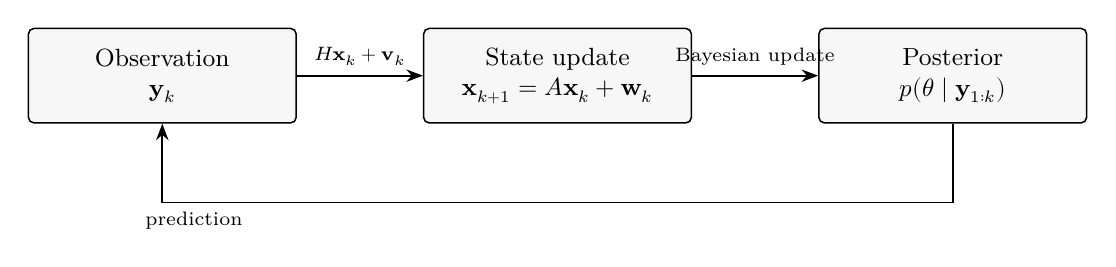
\begin{tikzpicture}[
  node distance=13mm and 16mm,
  box/.style={draw, rounded corners=2pt, minimum width=34mm, minimum height=12mm,
              align=center, line width=.55pt, font=\small},
  arrow/.style={-{Stealth[length=2.1mm]}, line width=.6pt},
]
  \node[box, fill=gray!6] (obs) {Observation\\$\mathbf{y}_k$};
  \node[box, fill=gray!6, right=of obs] (state) {State update\\$\mathbf{x}_{k+1}=A\mathbf{x}_k+\mathbf{w}_k$};
  \node[box, fill=gray!6, right=of state] (post) {Posterior\\$p(\theta\mid\mathbf{y}_{1:k})$};

  \draw[arrow] (obs) -- node[above, font=\scriptsize] {$H\mathbf{x}_k+\mathbf{v}_k$} (state);
  \draw[arrow] (state) -- node[above, font=\scriptsize] {Bayesian update} (post);
  \draw[arrow] (post.south) -- ++(0,-10mm) -|
    node[pos=.48, below, font=\scriptsize] {prediction} (obs.south);
\end{tikzpicture}
\end{document}
